\documentclass[]{article}

% Imported Packages
%------------------------------------------------------------------------------
\usepackage{amssymb}
\usepackage{amstext}
\usepackage{amsthm}
\usepackage{amsmath}
\usepackage{enumerate}
\usepackage{fancyhdr}
\usepackage[margin=1in]{geometry}
\usepackage{graphicx}
\usepackage{extarrows}
\usepackage{setspace}
%------------------------------------------------------------------------------

% Header and Footer
%------------------------------------------------------------------------------
\pagestyle{plain}  
\renewcommand\headrulewidth{0.4pt}                                      
\renewcommand\footrulewidth{0.4pt}                                    
%------------------------------------------------------------------------------

% Title Details
%------------------------------------------------------------------------------
\title{SFWR ENG 3A04\\Deliverable \#2\\High-Level System Design}
\author{Jonathan Yu\\Samuel Jackson\\Bill Chen\\Fiona Hu\\Nikita Jagora}
\date{}                               
%------------------------------------------------------------------------------

% Document
%------------------------------------------------------------------------------
\begin{document}

\maketitle	

\section{Introduction}
\label{sec:introduction}

\subsection{Purpose}
\label{sec:purpose}

The purpose of this document is to describe the software architecture of the WhoDatDog mobile application. This document describes the hierarchy and structure of the system's components in terms of its' classes, by defining both each class of the system and the interractions between these classes. This document is intended for use by software design and system support personnel.

\subsection{System Description}
\label{sec:sysdescription}

The WhoDatDog system is a mobile application developed for mobile devices running a Google Android operating system of version 8.4.2 or higher. This system's primary function is to enable a user to identify the breed of a dog they may find in their immediate, physical environement. Additionally, the system enables users to search for locations where they may purchase or adopt a dog in their vicinity, i.e. pet stores, dog pounds, etc., and to create posts on the Twitter social network, to describe to other users a dog they have identified and the geographic location where they have seen it.\\\\In order to accomplish these functions, the WhoDatDog software system employs a hierarchial system architecture which includes user interfaces at the top level, system controllers at the bottom level, and system memory at the lower level. In particular, the system's memory contains three so-called "expert" systems which are used for dog breed identification, and the system also uses external systems in the form of Twitter and Google Maps plugins.

\subsection{Overview}
\label{sec:overview}

This contents of this document are organized into 6 sections, including Section 1, the introduction. Sections 2-5 which describe and define the software structure of the system in a different aspect.\\Section 2 contains use case diagrams of the system, which describe the external actors (i.e. users, etc.) and internal system software classes and interactions needed for the system to perform a particular functional system requirements.\\Section 3c contains an analysis class diagram, which identifies the controller, storage entity, and user/system interface boundary classes in the system and graphically displays how these classes are interconnected.\\Section 4 contains descriptions of the system architecture design. For both the entire system and all subsystems, this section describes the architecture design used and provides a justification of the design's use and a graphical diagram of the design.\\Section 5 of the document contains class responsibility collaboration (CRC) cards for all of the classes used in the system. Each card contains the name of the class it describes, and a brief description of the class's own responsibilities and the other classes it collaborates with.\\Though it does not describe the system, Section 5 states the division of labor among the authors of this document.

\section{Analysis Class Diagram}
\label{sec:analysisclassdiagram}

\begin{figure}[!ht]
\centering
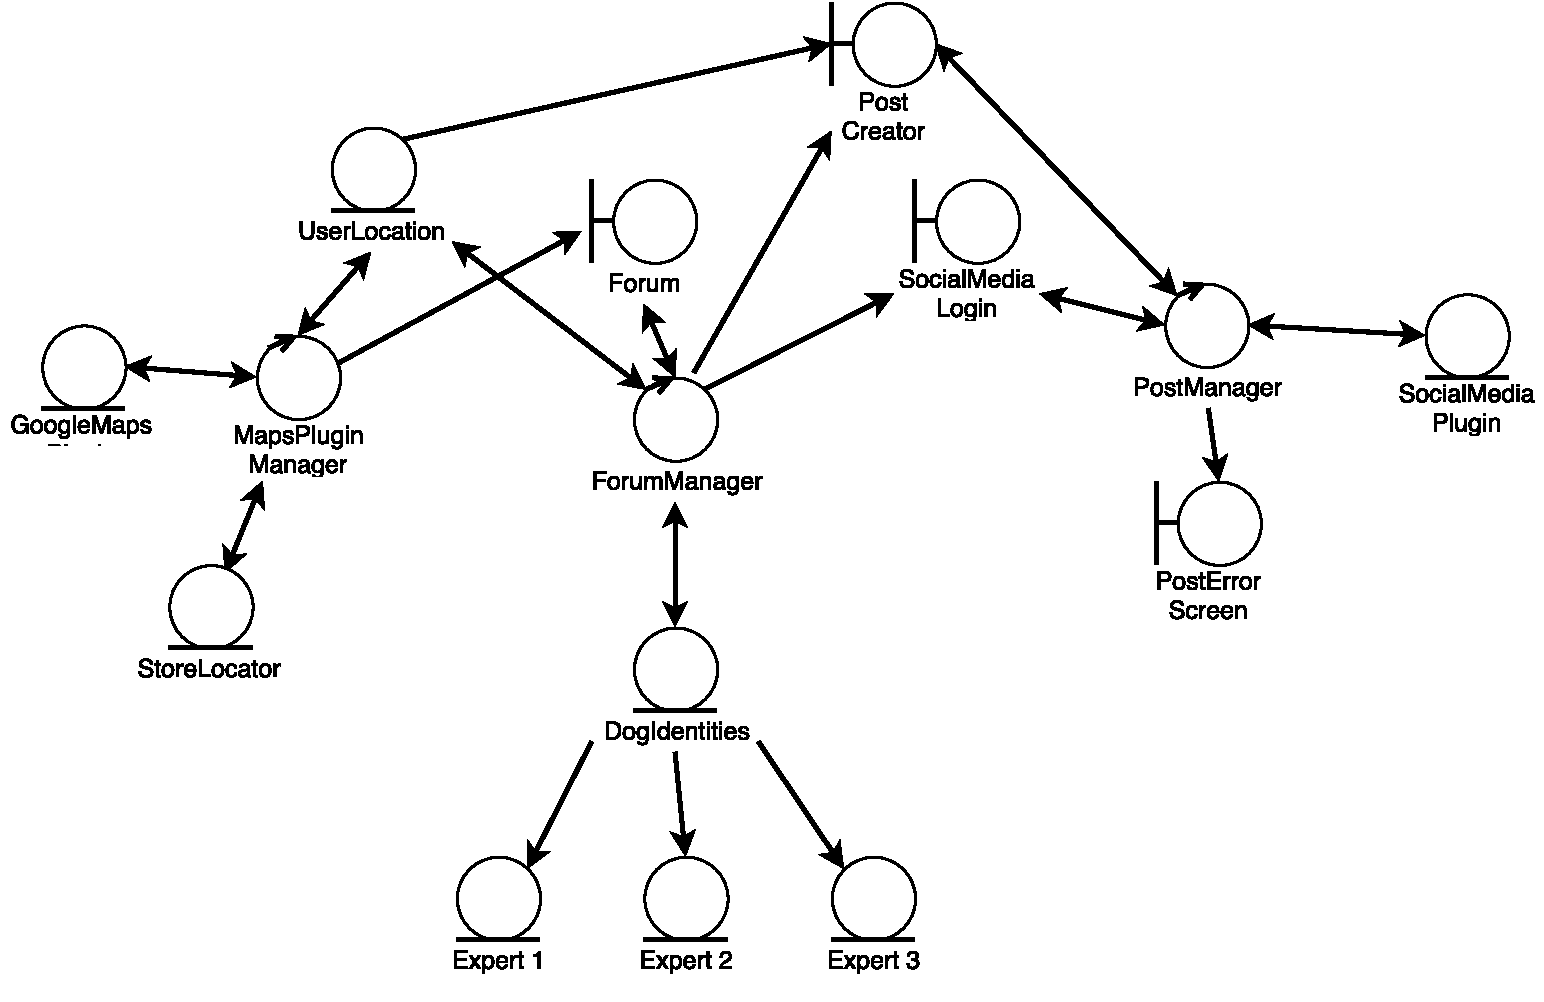
\includegraphics[width=\textwidth]{3A04_D2_Analysis_Class_Diagram.pdf}
\caption{\label{fig:analysisclassdiagram}An analysis class diagram of the WhoDatDog system.}
\end{figure}

\begin{itemize}
\item \textbf{Forum:} Boundary Class: Used as the main form of communication between the user and the system. Users can write text input to the forum, which the system will interpret and reply to.
\item \textbf{ForumManager:} Controller Class: Handles communication to and from the forum and the rest of the system.
\item \textbf{DogIdentities:} Entity Classes: Contains information regarding dog breeds. Connected to the three Expert entity sub-classes. This class receives a list of dog characteristics as input from the ForumManager class and returns a dog breed as input.
\item \textbf{Experts 1, 2 and 3:} Entity Classes: Each Expert contains information regarding a dog characteristic. When the DogIdentities class receives a request to identify a dog based on a list of characteristics, those characteristics are matched against those found in the Expert classes to determine the dog's breed.
\item \textbf{GoogleMaps:} Entity Class: Uses Google  Maps API Plugin as an entity from which geographical coordinates can be obtained.
\item \textbf{UserLocation:} Entity Class: Contains the user's current geographical location. Can optionally be used in the Post Creator class.
\item \textbf{StoreLocator:} Entity Class: Contains the geographical locations of pet stores, dog kennels, pounds, etc. locations near the user's own where the user may purchase/adopt a dog.
\item \textbf{MapsPluginManager:} Controller Class: Manages the interractions between the GoogleMaps, UserLocation, and StoreLocator classes. Can write responses to the Forum class regarding nearby stores.
\item \textbf{SocialMediaLogin:} Boundary Class: Prompts the user to enter their social media username and password.
\item \textbf{PostCreator:} Boundary Class: Used as a system interface through which the user can create a social media post. Also takes geographical information from the UserLocation class to use in the post.
\item \textbf{PostErrorScreen:} Boundary Class: Displayed if there is a communication error either with the social media post or the user's login credentials.
\item \textbf{SocialMediaPlugin:} Entity Class: A plugin for the Twitter social network service. Used as an entity class to access social network functionality such as the ability to create and publish posts.
\item \textbf{PostManager:} Controller Class: Manages the interractions between the PostCreator, SocialMediaLogin, PostErrorScreen, and SocialMediaPlugin classes.
\end{itemize}

\end{document}